\chapter{Parameter Lock Record  Page:}
The RLCK Page is used to record Parameter Locks in real-time. If the sequencer is running, any parameter changes on the MD will be recorded.\\
\\
\fbox{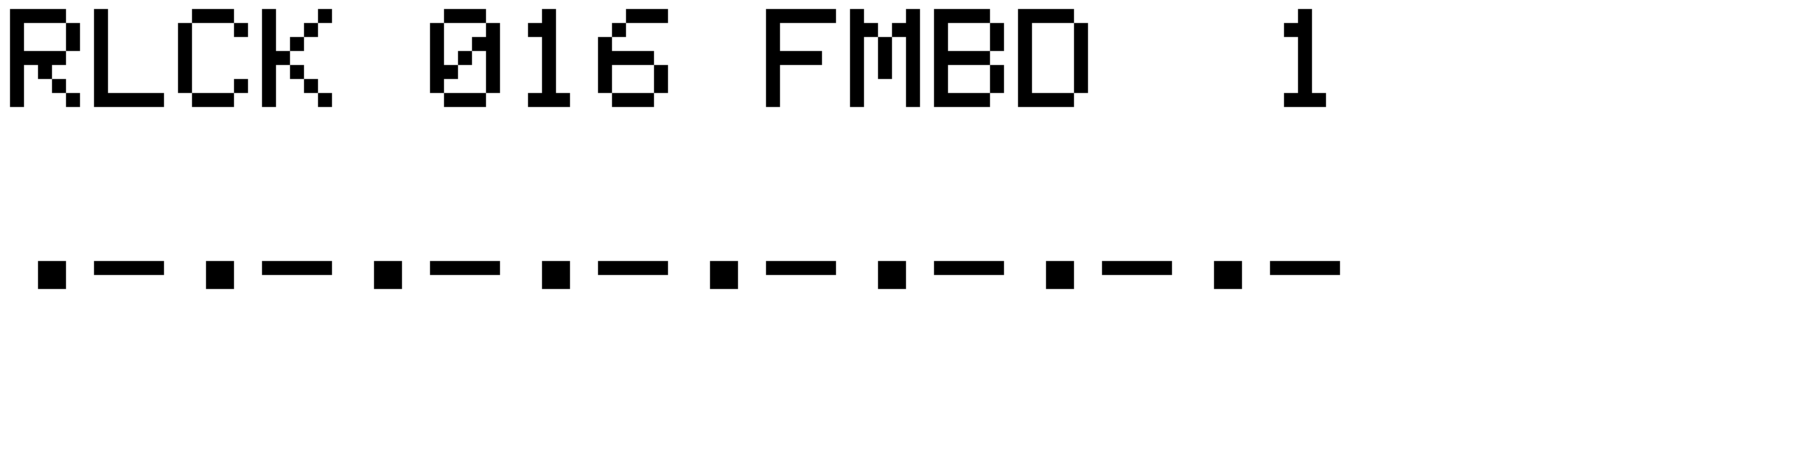
\includegraphics[scale=.40]{rlck_page_init.png}}\\
\textit{To enter the RLCK Page: Enter the RTRK Edit mode by pressing \textbf{[ Encoder 2 ]} from the Grid Page. Press the \textbf{[ Save ]} button to enter RLCK mode.}\\
\\
For each track parameter locks are automatically MIDI learnt. If a free parameter lock slot is available, it will automatically be assigned to the last Parameter received. \\
\\
When in RLCK Page, the current sequencer Track will automatically change according to the track of the last MD Parameter modified. 
\subsection{Clearing:}
To clear the current track of all parameter locks, press the \textbf{[ Write ] }(top right)\\
\\To clear all MD tracks of all parameter locks,  press \textbf{[ Shift2 ] + [ Write ]}
